\section{Modern applications}

Key characteristics of modern applications include:
\begin{itemize}
    \item \textit{Compute-intensiveness}: they will demand significant computational resources, necessitating optimized hardware and software regardless of their application domain.
    \item \textit{Connectivity}: these applications will be interconnected, either wired or wirelessly, and will often be online—globally interconnected through the Internet.
    \item \textit{Physical entanglement}: they will be embedded within and capable of interacting with the physical world, not only observing but also controlling their environment. 
    \item \textit{Intelligence}: these applications will possess the capability to interpret noisy, incomplete, analog, or remote data from the physical world, allowing for smarter interactions and decision-making.
\end{itemize}
The ongoing integration of the digital and physical worlds will be driven by advances in cognitive computing, big data analytics, and data mining.
\begin{figure}[H]
    \centering
    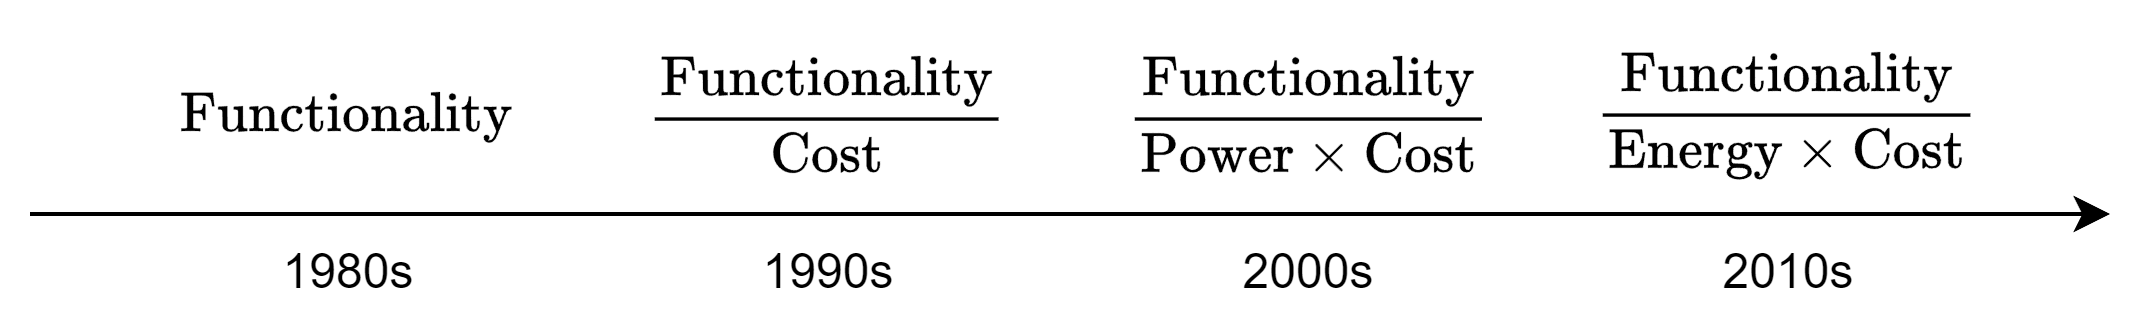
\includegraphics[width=0.75\linewidth]{images/time.png}
    \caption{Industry requirements}
\end{figure}
While the number of transistors in modern systems can continue to increase, a key challenge is that we cannot power all of them simultaneously. 
This limitation drives the need for innovative approaches to using extra transistors more efficiently. 
Additionally, heterogeneous processing combined with aggressive power management is crucial for optimizing performance across various tasks.

\paragraph*{Transistors}
As transistors shrink in size, several challenges emerge. 
Process variation, physical failures, and aging mechanisms can degrade device performance over time. 
With very-large-scale integration, packing more transistors into smaller spaces increases power density, which in turn creates thermal issues. 
Furthermore, traditional communication subsystems struggle to provide adequate power-performance trade-offs in these densely packed systems. 

\paragraph*{Silicon}
Despite silicon being a relatively good thermal conductor, large chips can still experience significant temperature gradients. 
One practical solution involves dividing the chip into concentric rings and applying dynamic voltage and frequency scaling to each region. 
By fine-tuning voltage and frequency for each ring, it becomes possible to optimize performance while maintaining thermal balance.

\paragraph*{Frequency}
Modern systems address power management by partitioning chips into independent islands that operate at different voltage and frequency levels. 
This approach allows sections of the chip to be dynamically turned off when not in use, a process known as power gating. 

\subsection{Cooling}
Air cooling, while common, suffers from a low heat transfer coefficient, poor chip temperature uniformity, and requires large heat sinks and air ducts.
It is also noisy and expensive to maintain. 
Water cooling offers an improvement, more uniform chip temperatures, smaller heat sinks, and fewer fans. 
Water cooling also allows for potential heat recovery, though it requires large pumps to function effectively.

Two-phase cooling systems present an even more efficient solution. 
They provide better chip temperature uniformity, and smaller pumps, along with isothermal coolant. 
However, two-phase cooling systems suffer from low pump efficiency and reliability issues.